\chapter{Risultati}

Questo capitolo presenta i risultati degli esperimenti di rilevamento delle allucinazioni. Vengono analizzate le prestazioni dei probe lineari e l'efficacia dell'allineamento cross-model.

\section{Analisi PCA delle Attivazioni}

Per visualizzare la separabilità degli stati allucinati e non allucinati, è stata eseguita l'Analisi delle Componenti Principali (PCA) sulle attivazioni.

\begin{figure}[h]
    \centering
    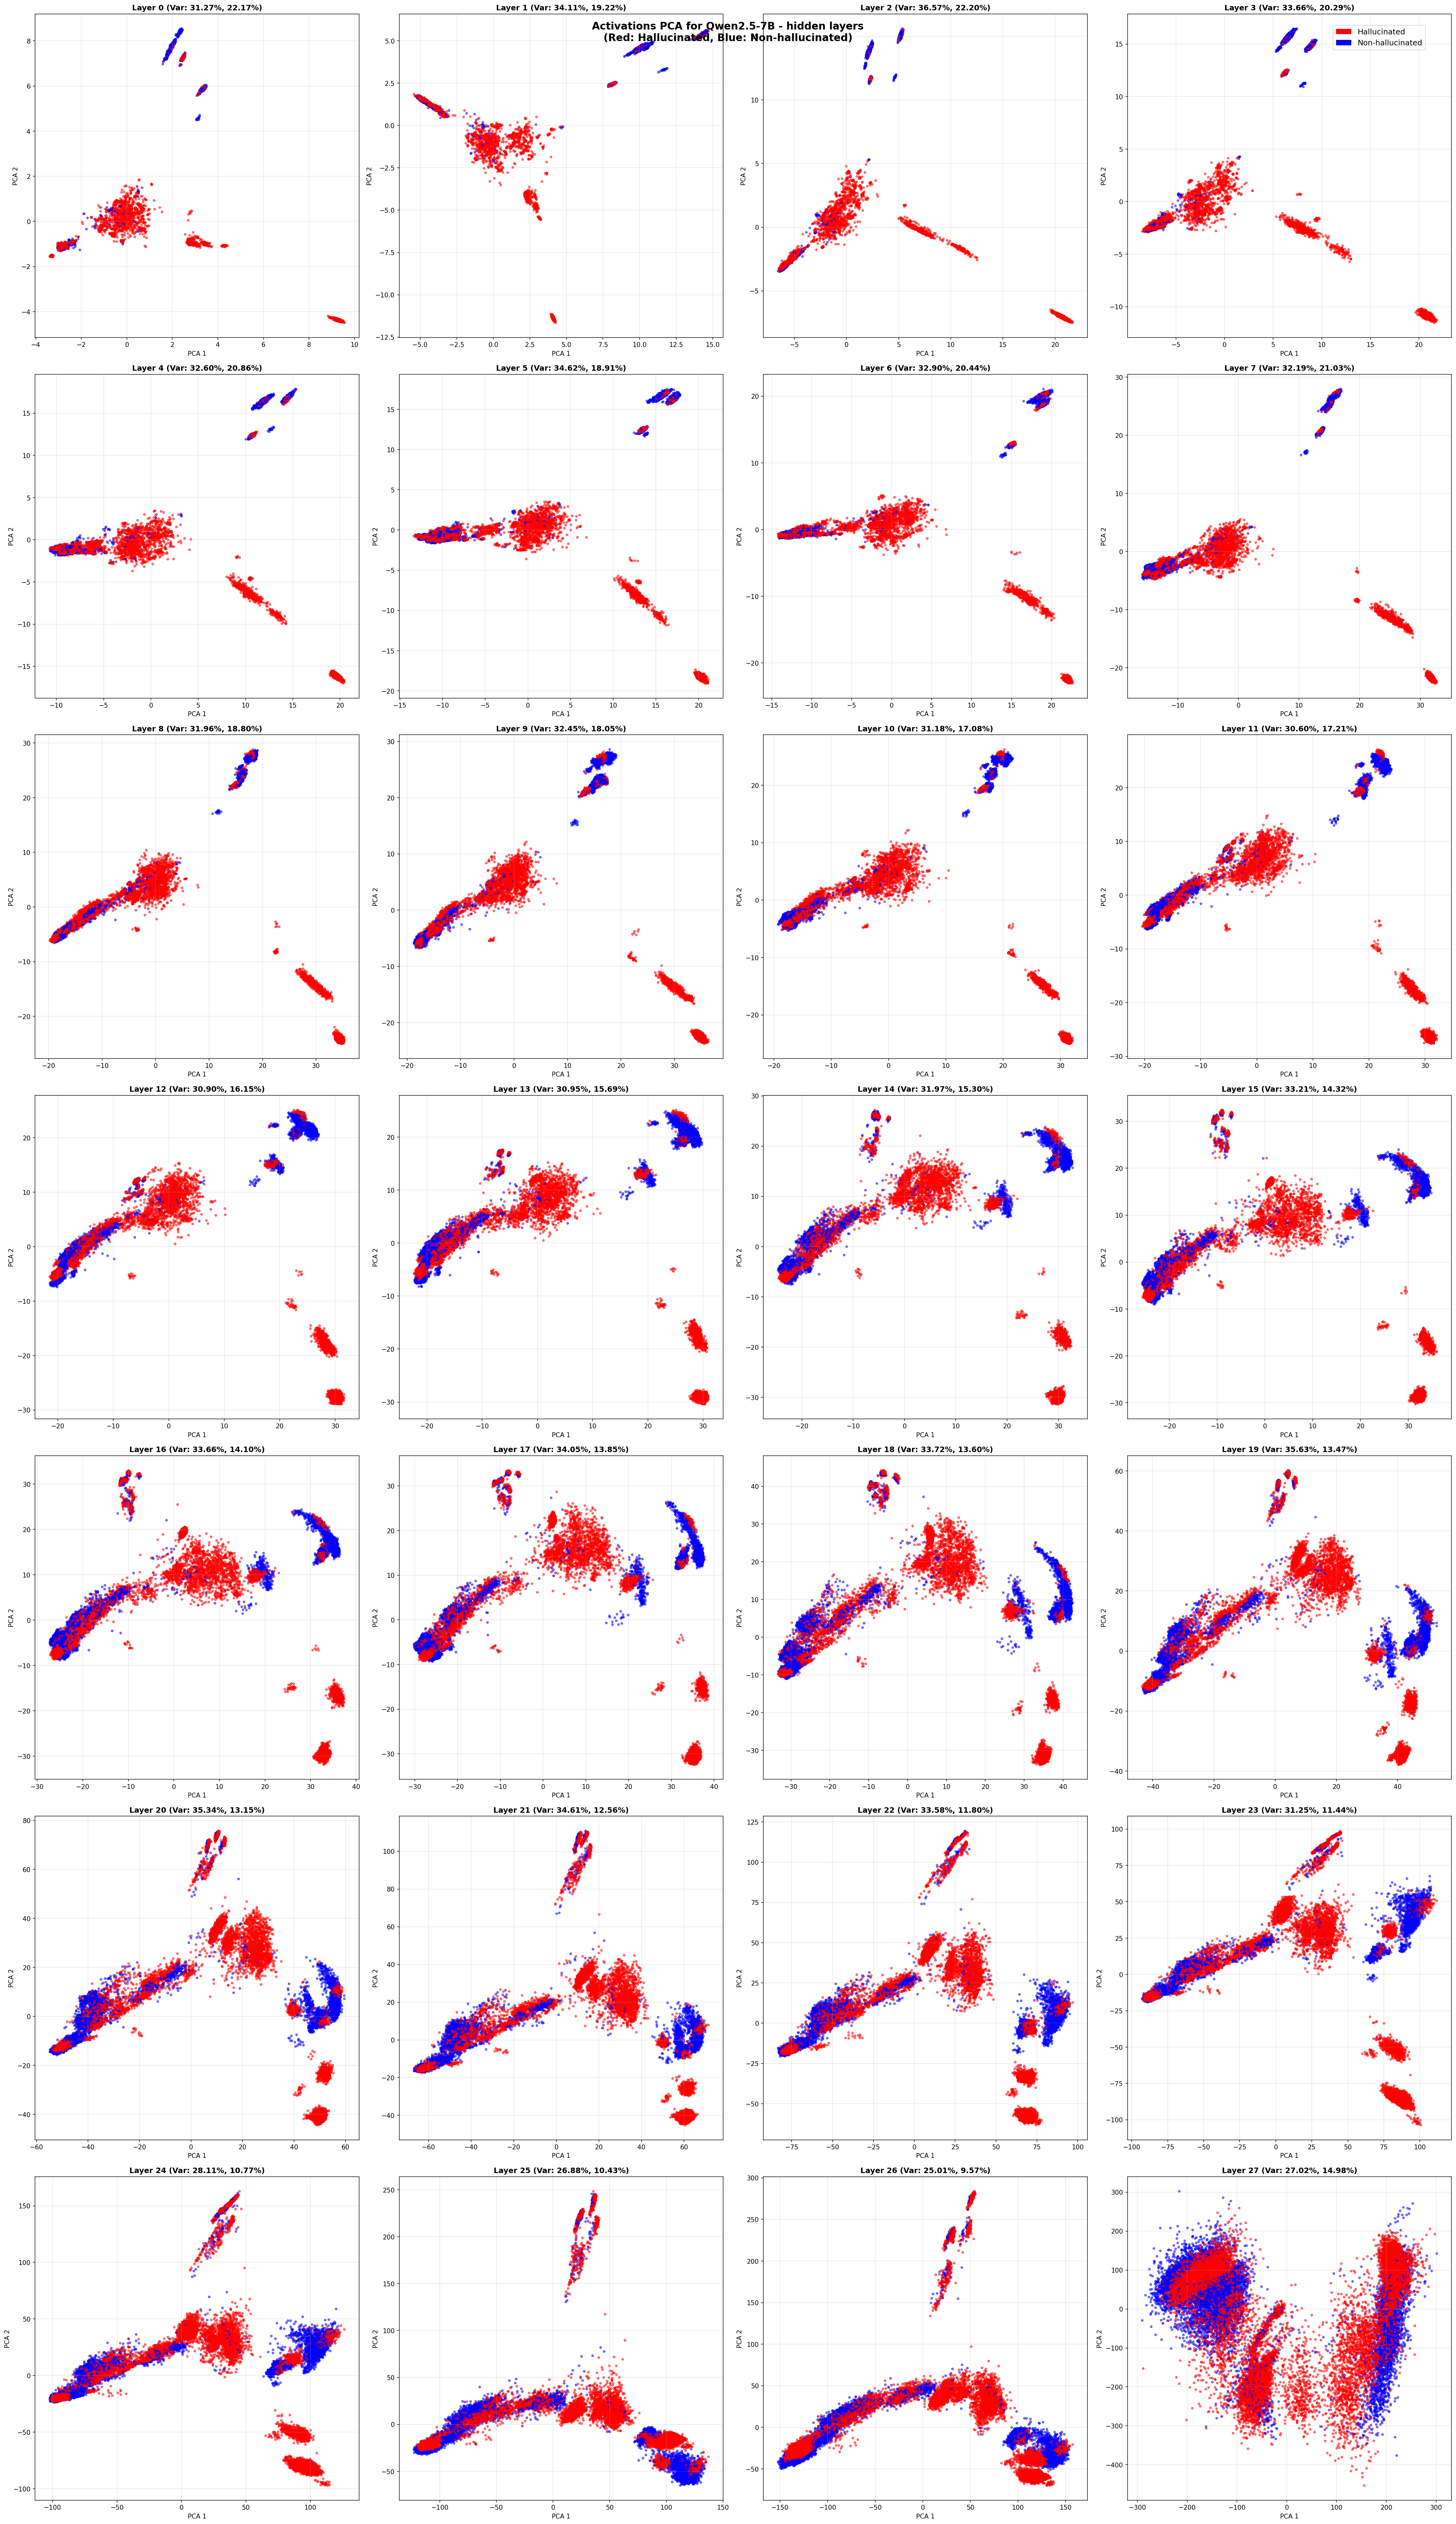
\includegraphics[width=0.45\textwidth]{images/plots/Qwen2.5-7B_belief_bank_hidden_activations_PCA.png}
    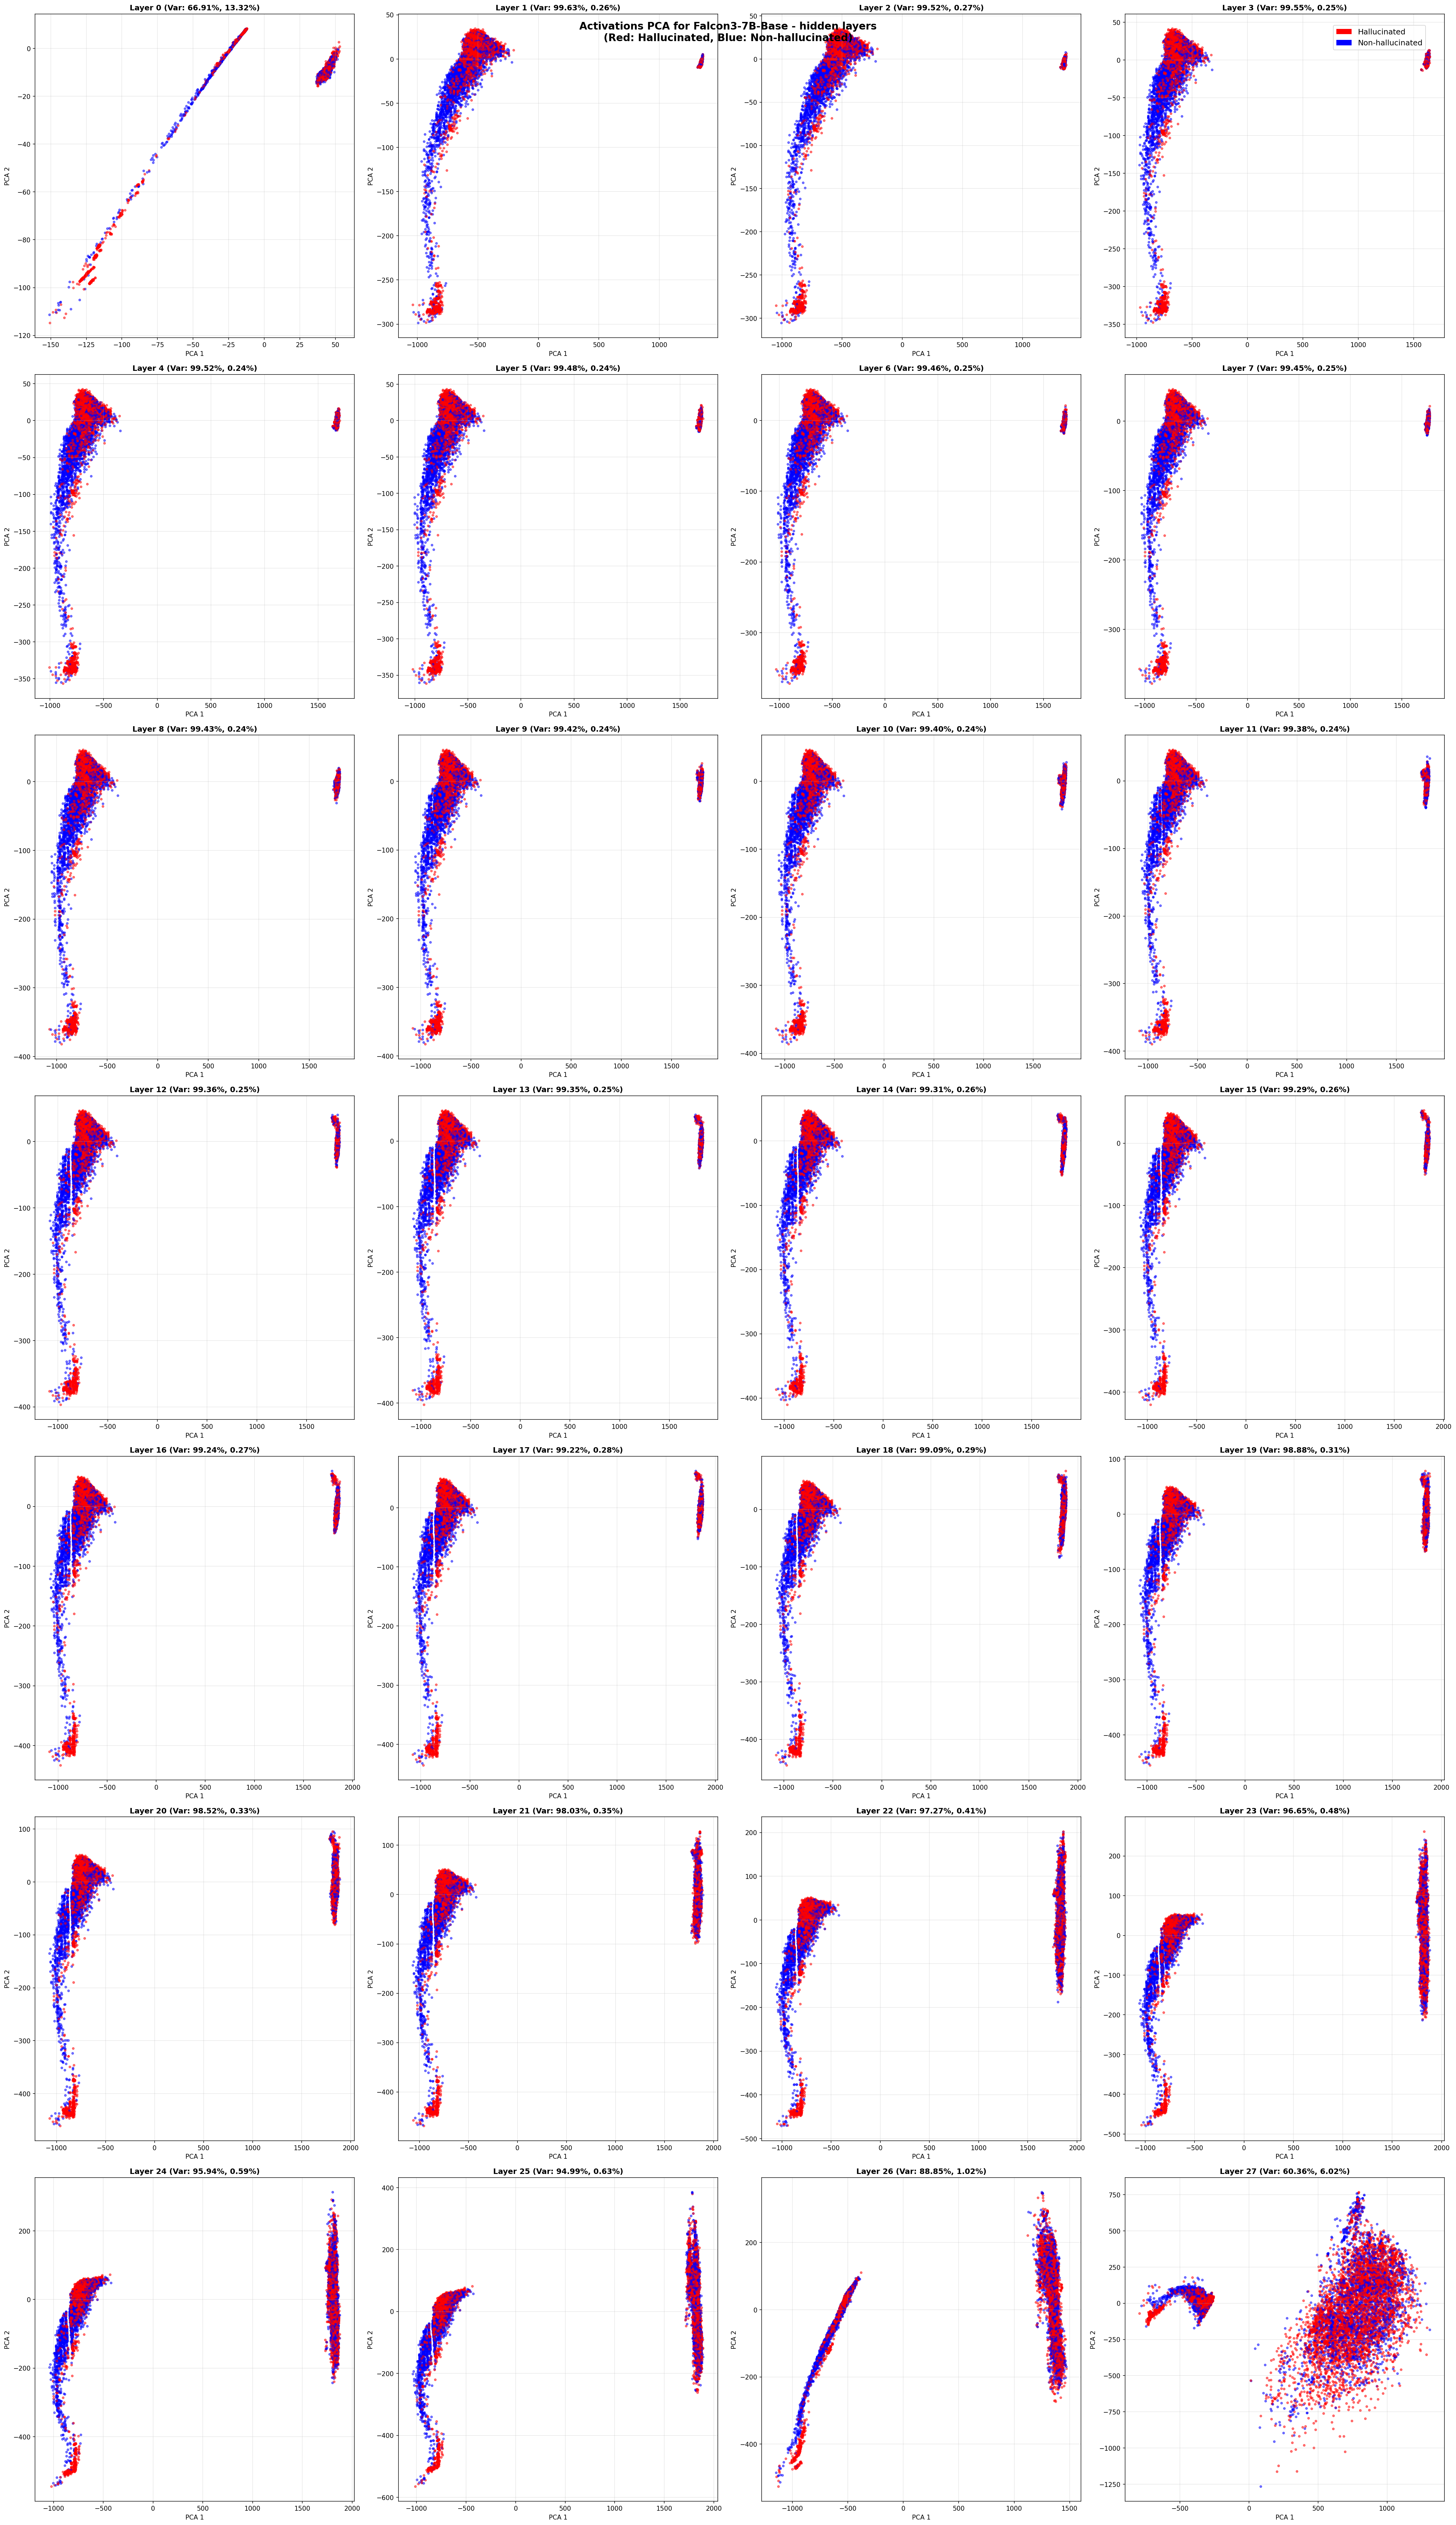
\includegraphics[width=0.45\textwidth]{images/plots/Falcon3-7B-Base_belief_bank_hidden_activations_PCA.png}
    \caption{PCA delle Attivazioni Hidden Layer per Qwen2.5-7B (sinistra) e Falcon3-7B-Base (destra). I punti rossi indicano le allucinazioni.}
    \label{fig:pca_hidden}
\end{figure}

Come mostrato in Figura \ref{fig:pca_hidden}, esiste una notevole separazione tra le due classi nello spazio delle attivazioni, in particolare per il modello Qwen. Nei laayer intermedi e finali è possibile osservare diversi cluster. Per il modello Falcon, la separazione è meno marcata ma ancora evidente in alcuni layer.

\section{Risultati Quantitativi}

Sono state valutate le prestazioni dei probe in due scenari:
\begin{enumerate}
    \item \textbf{Scenario 1}: Qwen2.5-7B come Teacher $\rightarrow$ Falcon3-7B-Base come Student.
    \item \textbf{Scenario 2}: Falcon3-7B-Base come Teacher $\rightarrow$ Qwen2.5-7B come Student.
\end{enumerate}

\subsection{Scenario 1: Qwen $\rightarrow$ Falcon}

In questo scenario, il probe è stato addestrato sulle attivazioni di Qwen. Qwen ha raggiunto un'elevata accuratezza nel rilevare le proprie allucinazioni.

\begin{table}[h]
\centering
\begin{tabular}{|l|c|c|c|c|}
\hline
\textbf{Tipo Layer} & \textbf{Acc Teacher} & \textbf{Acc Student} & \textbf{F1 Teacher} & \textbf{F1 Student} \\ \hline
Attention & 0.9880 & 0.7328 & 0.9897 & 0.7642 \\ \hline
MLP & 0.9889 & 0.6546 & 0.9905 & 0.7245 \\ \hline
Hidden & 0.9895 & 0.7004 & 0.9910 & 0.7447 \\ \hline
\end{tabular}
\caption{Risultati per lo Scenario 1 (Qwen $\rightarrow$ Falcon)}
\label{tab:results_qwen_falcon}
\end{table}

I risultati nella Tabella \ref{tab:results_qwen_falcon} mostrano che mentre il probe è estremamente efficace sul Teacher (Qwen), le prestazioni calano significativamente quando applicato allo Student allineato (Falcon), con un'accuratezza che varia dal 65\% al 73\%.

\subsection{Scenario 2: Falcon $\rightarrow$ Qwen}

Nello scenario inverso, Falcon è stato utilizzato come Teacher.

\begin{table}[h]
\centering
\begin{tabular}{|l|c|c|c|c|}
\hline
\textbf{Tipo Layer} & \textbf{Acc Teacher} & \textbf{Acc Student} & \textbf{F1 Teacher} & \textbf{F1 Student} \\ \hline
Attention & 0.8930 & 0.6534 & 0.9110 & 0.7197 \\ \hline
MLP & 0.7970 & 0.6283 & 0.8270 & 0.7045 \\ \hline
Hidden & 0.8737 & 0.6530 & 0.8944 & 0.7231 \\ \hline
\end{tabular}
\caption{Risultati per lo Scenario 2 (Falcon $\rightarrow$ Qwen)}
\label{tab:results_falcon_qwen}
\end{table}

La Tabella \ref{tab:results_falcon_qwen} indica che Falcon è un Teacher meno efficace, con un'accuratezza di base inferiore. Anche il trasferimento a Qwen è limitato, con accuratezze intorno al 62-65\%.

\section{Matrici di Confusione}

Gli errori sono stati ulteriormente analizzati utilizzando le matrici di confusione.

\begin{figure}[h]
    \centering
    \includegraphics[width=0.45\textwidth]{images/plots/confusion_matrix_hidden_Teacher_Qwen2.png}
    \includegraphics[width=0.45\textwidth]{images/plots/confusion_matrix_hidden_Falcon3-7B-Base_on_Qwen2.png}
    \caption{Matrici di Confusione per Hidden Layers. Sinistra: Qwen (Teacher). Destra: Falcon su Qwen (Student).}
    \label{fig:cm_hidden}
\end{figure}

La Figura \ref{fig:cm_hidden} illustra che l'applicazione cross-model comporta un numero maggiore di Falsi Positivi e Falsi Negativi rispetto all'autovalutazione del Teacher.


Qwen è un modello da 28 layer ciascuno con una hiddensize di 3584, mentre Falcon ha 28 layer con una hiddensize di 3,072.
Questo potrebbe suggerire che usare un modello Teacher più grande e complesso aiuti a catturare rappresentazioni più ricche per il rilevamento delle allucinazioni, facilitando il trasferimento allo Student.